\documentclass[12pt]{article}
\usepackage{amsmath, amssymb, amsthm, graphicx, epsfig, fancyhdr, graphicx}
\usepackage{algorithm}
\usepackage[noend]{algpseudocode}
\usepackage[utf8]{inputenc}

\title{Math 240 Overleaf Form} 
\author {Laouen belloli}

\setlength{\headheight}{28pt}
\pagestyle{fancy}
\fancyhf{}
\fancyhead[R]{Laouen Belloli \\ Automatic creation of Metabolic Network in PDEVS}
\fancyfoot[C]{\thepage}


\begin{document}

\section*{Modelado de las reacciones}

Mirando el modelo en DEVS armado por Roxana Djafarzadeh de Glycolysis, pude ver que todos los pasos (Steps 1-10, los cuales modelan distintas reacciones), tienen la misma estructura. Esta estructura es parecida a la que hablamos la última vez por Skype en donde hay reactantes y lo que creo que se llaman ensimas y se obtiene como output los productos. \\

Por otro lado, estuve leyendo el manual de SBML y en el manual habla de "rate" como una función que indica el tiempo en que tarda la reacción en terminar y "stoichiometry" como una ecuación que indica la relación de cantidades entre los reactantes y los productos, la cual tiene que mantener una equivalencia de masas, o sea, la misma cantidad de moléculas con las que comienza la reacción es la cantidad de moléculas que va a devolver en los productos.

Comprendí la idea de rate y stoichiometry pero algunas dudas tengo al respecto que necesitaría sacarme. \\

Para el modelo de glycolysis, el rate está definido constantemente en 0 y el stoichiometry es la ecuación donde los coeficientes son siempre 1. \\

$k*(r_1 + r_2 + ... + r_n) = k*(p_1 + p_2 + ... + p_m)$ \\

pero esto podría ser algo como: \\

$k*(a_1*r_1 + a_2*r_2 + ... + a_n*r_n) = k*(b_1*p_1 + b_2*p_2 + ... + b_m*p_m)$ \\

donde los $a_i$ $b_j$ son coeficientes, o sea, numeros naturales mayores que 0.

Me gustaría charlar sobre esto y ver como está expresado esto en el archivo SBML así puedo ver bien como interpretar el archivo. además ver como manejar esta ecuación (lo mismo me gustaría ver con el rate). En el modelo de glycolysis es demasiado sencillo como para comprender el caso general.

\newpage
\subsection*{Primer apouch al modelo de las reacciones}
El modelo que tengo inplementado hasta el momento, y que seguro esta mal porque tome decisiones sobre las cosas mencionadas anteriormente, de las cuales tengo dudas, es el siguiente: \\

Reaction = $< S, X, Y, \delta INT, \delta EXT, ta, \lambda >$

\begin{itemize}

\item S = $\{ \{ (molecula, cantidad) \ | \ molecula \in MOLECULAS, \ cantidad \in [0..\infty] \} \}$
\item X = $\{ (molecula, cantidad) \ | \ molecula \in MOLECULAS, \ cantidad \in [0..\infty] \}$
\item Y = $\{ (molecula, cantidad) \ | \ molecula \in MOLECULAS, \ cantidad \in [0..\infty] \}$
\end{itemize}

\begin{algorithm}[h]
\begin{algorithmic}[h]
\Function{$\delta$int}{ }
\State $products.setAllInZero()$
\State $reactants.setAllInZero()$
\State $enzymes.setAllInZero()$
\EndFunction
\end{algorithmic}
\end{algorithm}

\begin{algorithm}[h]
\begin{algorithmic}[h]
\Function{$\delta$ext}{ molecule $m$ }
\State
\For {$r \in reactants$}
\If {$r.name == m.name$}
\State $r.amount \leftarrow (r.amount + m.amount)$
\EndIf
\EndFor
\State
\If{$thereIsEnoughElements(reactants,enzymes)$}
\State $k \leftarrow maximumAvailable(products, enzymes, stoichiometry)$
\State
\For {$r \in reactants$}
\State $r \leftarrow (r - k*calculateStoichiometry(r, stoichiometry))$
\EndFor
\State
\For {$p \in products$}
\State $p.amount \leftarrow k*calculateStoichiometry(p, stoichiometry)$
\EndFor
\EndIf
\EndFunction
\end{algorithmic}
\end{algorithm}

\begin{algorithm}[h]
\begin{algorithmic}[h]
\Function{ta}{ }
\State
\If {$thereIsProductsToSend(products)$}
\State $nextInternalTransition \leftarrow calculateRate(rate)$
\Else
\State $nextInternalTransition \leftarrow \infty$
\EndIf
\EndFunction
\end{algorithmic}
\end{algorithm}

\begin{algorithm}[h]
\begin{algorithmic}[h]
\Function{$\lambda$}{ }
\State $return append(products, reactants)$
\EndFunction
\end{algorithmic}
\end{algorithm}

\textbf{notas:}\\
\begin{itemize}
\item $MOLECULAS$ es el conjunto de todas las moleculas existentes en el modelo.
\item Las funciones $calculateStoichiometry$, $calculateRate$, $maximumAvailable$ son en general las que tendríamos que discutir bien como funcionan y además son lo principal. Necesito discutir estas funciones más que nada. Aunque como dije antes este modelo seguro esta mal o le faltan partes.
\item Las funciones $append$ y $setAllInZero$ hacen lo que el nombre indica.
\end{itemize}

\newpage
El siguiente grafico muestra la estructura de un modelo atomico reaction:

\begin{figure}[h!]
 \centering
  \includegraphics[width=1\textwidth]{reaction.jpg}
 \caption{estructura interna de una clase reaction. Los triángulos blancos marcan herencia, por eso no tienen cardinalidad, los triángulos negros marcan pertenencia y tienen anotada la relación de cardinalidades.}
\end{figure}

\newpage
\section*{Modelado de los pathway o network}

En el modelo de Glycolysis no hay un modelo acoplado armado, hay unos graficos que muestran como seria, eso no está bueno porque no puedo validar mis resultados, pero además tampoco es bueno, porque una de las cosas que quería ver en ese modelo era como se asignaban los reactantes a las reacciones. \\

Leí que (aca me puedo equivocar mucho porque no es mi campo) depende de la cercanía, los reactantes se chocan o están muy cerca junto con las enzimas y en ese momento ocurre una reacción.  

Teniendo esto en cuenta, el camino de las 10 reacciones que aparece en el modelo de glycolysis parece un tanto raro ya que una reacción $step_i$ le da los elementos en la mano a la otra reacción siguiente en el camino $step_{i+1}$ conectando el output de una reacción al input de otra para armar este camino de 10 pasos. Esta no me parece que sea la opción correcta (de nuevo puedo estar muy equivocado en esta parte).

Por otro lado, como es un camino unidireccional, una ves que una reacción se lleva a cabo, no se resetea la enzima (en el modelo de Roxana), lo cual me hace ruido. \\

Mi idea para esto (sin saber mucho) es que hay que hacer un modelo controlador el cual recibe las moléculas ya sea porque vienen como input externo o porque una reacción dio productos. Todas las moléculas van a parar en primera instancia a este controlador y luego él es quien decide a que reacciones darle cada molécula o al output y cuanto darle.

Aca me surgen mil dudas de con que criterio debería hacer esto, ya que no tengo idea como es, mirando lo que investigué en internet, es un tema de cercanía, entonces habría que modelar en que punto del espacio esta cada molécula y como se va moviendo (supongo que con probabilidades) y que decida cuando todos los reactantes de una reacción están cerca entonces que suceda. Digo esto como no digo nada y necesito realmente discutir esta parte.

\newpage
Aca pongo un grafico entonces de como seria en grandes rasgos el modelo acoplado. Tengo más graficos de como son cada modelo atomico pero creo que no tiene sentido mostrarlo aca, ya que los modelos atomicos hay que discutir y terminarlos.


\begin{figure}[h!]
 \centering
  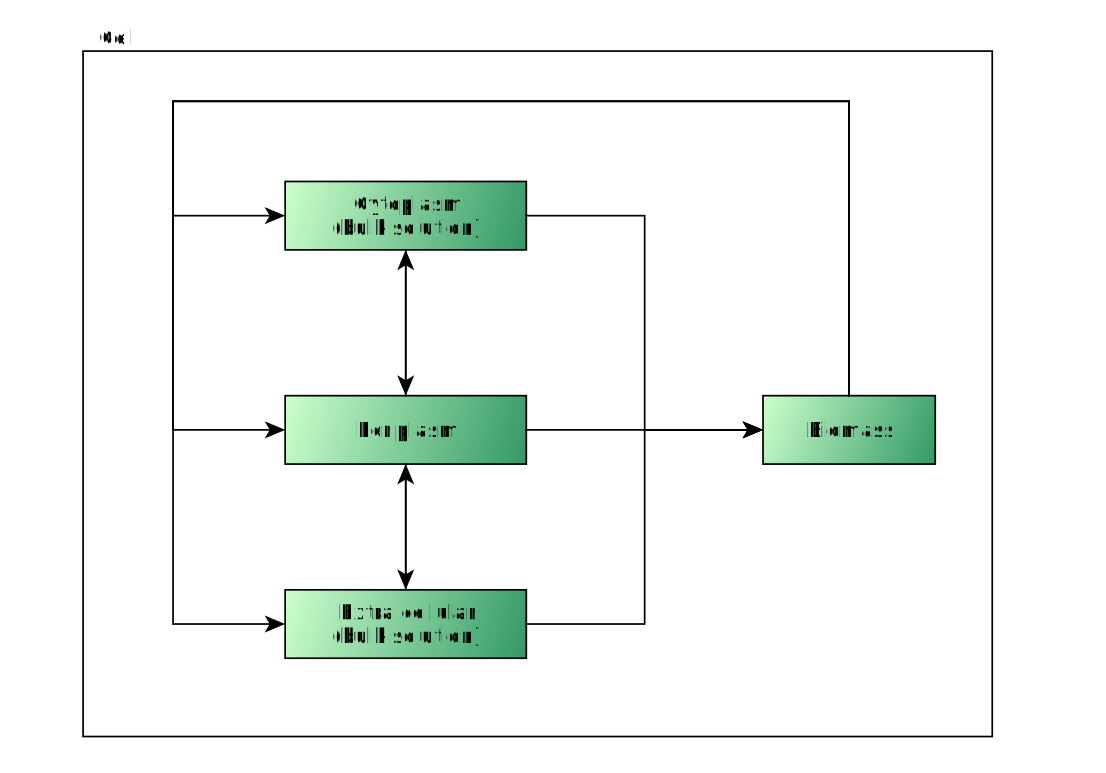
\includegraphics[width=1\textwidth]{coupled-model.jpg}
 \caption{coupled model.}
\end{figure}

\section*{Gran duda}
También estuve mirando que hay compartimentos y que las reacciones pueden pasar moléculas de un compartimento a otro. No sé esto si hay que modelarlo y en tal caso como hay que modelarlo. De nuevo necesito recibir algunas explicaciones de esto.

\section*{SBML}
Estuve leyendo el manual completo en la web y me descargue una librería tinyXML que incluí en el proyecto C++ para parsear el archivo SBML y anda perfectamente. Me devuelve el SBML en un objeto C++ DOM o sea padres e hijos anidados. Tengo que hacer unas funciones para interpretar las funciones matemáticas y el resto es ver como interpretar el archivo, Esto también necesito discutirlo.

Bueno, estos son mis avances hasta el momento tras unas semanas de leer mucho de muchas cosas.
Saludos !










  















\end{document}